\documentclass{sigchi}

% Use this command to override the default ACM copyright statement (e.g. for preprints). 
% Consult the conference website for the camera-ready copyright statement.


%% EXAMPLE BEGIN -- HOW TO OVERRIDE THE DEFAULT COPYRIGHT STRIP -- (July 22, 2013 - Paul Baumann)
% \toappear{Permission to make digital or hard copies of all or part of this work for personal or classroom use is 	granted without fee provided that copies are not made or distributed for profit or commercial advantage and that copies bear this notice and the full citation on the first page. Copyrights for components of this work owned by others than ACM must be honored. Abstracting with credit is permitted. To copy otherwise, or republish, to post on servers or to redistribute to lists, requires prior specific permission and/or a fee. Request permissions from permissions@acm.org. \\
% {\emph{CHI'14}}, April 26--May 1, 2014, Toronto, Canada. \\
% Copyright \copyright~2014 ACM ISBN/14/04...\$15.00. \\
% DOI string from ACM form confirmation}
%% EXAMPLE END -- HOW TO OVERRIDE THE DEFAULT COPYRIGHT STRIP -- (July 22, 2013 - Paul Baumann)


% Arabic page numbers for submission. 
% Remove this line to eliminate page numbers for the camera ready copy
% \pagenumbering{arabic}


% Load basic packages
\usepackage{balance}  % to better equalize the last page
\usepackage{graphics} % for EPS, load graphicx instead
\usepackage{times}    % comment if you want LaTeX's default font
\usepackage{url}      % llt: nicely formatted URLs

% llt: Define a global style for URLs, rather that the default one
\makeatletter
\def\url@leostyle{%
  \@ifundefined{selectfont}{\def\UrlFont{\sf}}{\def\UrlFont{\small\bf\ttfamily}}}
\makeatother
\urlstyle{leo}


% To make various LaTeX processors do the right thing with page size.
\def\pprw{8.5in}
\def\pprh{11in}
\special{papersize=\pprw,\pprh}
\setlength{\paperwidth}{\pprw}
\setlength{\paperheight}{\pprh}
\setlength{\pdfpagewidth}{\pprw}
\setlength{\pdfpageheight}{\pprh}
\usepackage{epstopdf}
\usepackage{graphicx}
\usepackage{caption}
\usepackage{subcaption}
\usepackage{float}
% Make sure hyperref comes last of your loaded packages, 
% to give it a fighting chance of not being over-written, 
% since its job is to redefine many LaTeX commands.
\usepackage[pdftex]{hyperref}

\hypersetup{
pdftitle={SIGCHI Conference Proceedings Format},
pdfauthor={LaTeX},
pdfkeywords={SIGCHI, proceedings, archival format},
bookmarksnumbered,
pdfstartview={FitH},
colorlinks,
citecolor=black,
filecolor=black,
linkcolor=black,
urlcolor=black,
breaklinks=true,
}



% create a shortcut to typeset table headings
\newcommand\tabhead[1]{\small\textbf{#1}}


% End of preamble. Here it comes the document.
\begin{document}

\title{Effect of Embodiment of Video Instructor on Student's Learning Process}

\numberofauthors{3}
\author{
  \alignauthor Jia-Shen Boon\\
    \affaddr{University of Wisconsin-Madison}\\
    \affaddr{1210 West Dayton Street}\\
    \affaddr{Madison, WI 53706, USA}\\
    \email{boon@cs.wisc.edu}\\
    %\affaddr{Optional phone number}
  \alignauthor Ke Ma\\
    \affaddr{University of Wisconsin-Madison}\\
    \affaddr{1210 West Dayton Street}\\
    \affaddr{Madison, WI 53706, USA}\\
    \email{kma@cs.wisc.edu}\\
    %\affaddr{Optional phone number}    
  \alignauthor Ayon Sen\\
    \affaddr{University of Wisconsin-Madison}\\
    \affaddr{1210 West Dayton Street}\\
    \affaddr{Madison, WI 53706, USA}\\
    \email{ayonsn@cs.wisc.edu}\\
    %\affaddr{Optional phone number}
}

\maketitle

\begin{abstract}
Faculty members are often busy with various research work and thus have little time to prepare lectures. Advances in technology offer a solution to this problem. That is, they can record the lectures and reuse them over semesters. It is common for these lecture videos to include an inset frame of the instructor giving the lecture. However, little research has been done to investigate the effect of these inset frames. In this study, we examined how the physical embodiment of the instructor in the inset frame impacts the learning process. Three types of embodiment were compared through an online between-participants experiment: lecture with no inset frame, lecture with an inset frame of a human instructor and lecture with an inset frame of a virtual agent instructor. The results showed a marginally significant difference between having some form of embodiment and having no embodiment in terms of learning performance.\end{abstract}

\keywords{
	video lecture; virtual agent; embodiment;% conference publications;
	%keywords should be separated by a semi-colon. \newline
	%\textcolor{red}{Optional section to be included in your final version, 
  %but strongly encouraged.}
}

%\textcolor{red}{Optional section to be included in your final version, 
%but strongly encouraged. On the submission page only the classifiers’ 
%letter-number combination will need to be entered.}


\section{Introduction}

Faculty members are usually very busy with various research work and other obligations. This provides them with little time to prepare lectures which is very important for the transfer of knowledge. Advances in technology expand the instructional options for the faculty and therefore offer a solution to the problem. That is, they can record these lectures and use the same recording every semester. These video lectures often include an inset frame of the instructor giving the lecture (Figure ~\ref{fig:mooc_inset}), presumably to improve the learning performance and experience of the students. We refer to these types of lectures as {\it personalized video lectures}. 

\begin{figure}
    \centering
    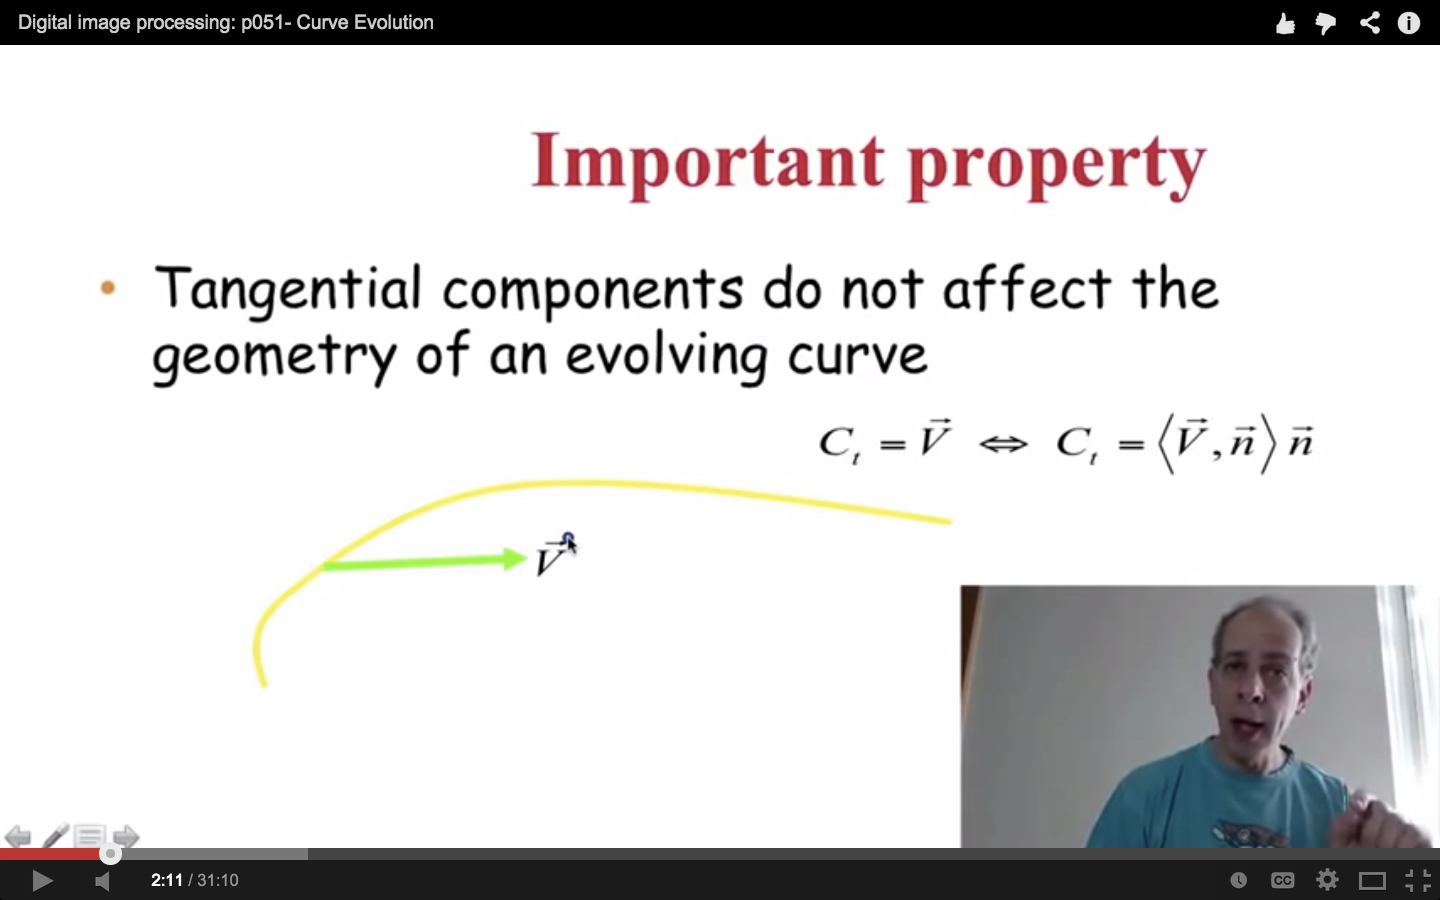
\includegraphics[width=0.3\textwidth]{Figures/mooc_inset.png}
    \caption{Lecture video of an online course with an inset frame of a human instructor \protect\cite{improc}.}
    \label{fig:mooc_inset}
\end{figure}

Although many online lectures do have this frame in their videos, anecdotally, the majority does not. It would cost much time and energy for the instructors to record these lectures again in order to include such frames. As virtual agents are known to be good at giving instructions, an alternative approach is to include an inset frame of a virtual agent. If this approach proves to be beneficial, people may automatically generate inset videos of such virtual agents in post-production for all online lectures that have been filmed without the instructors present in the videos. This would be much more cost-effective than recording the lectures again.

Our goal in this study is to investigate the role that the inset frame plays in the process of students learning from video lectures. Specifically, we seek to gain a better understanding of how the presence and absence of this inset frame as well as the embodiment of the instructor therein may influence the student's objective learning performance and subjective learning experience. By exploring these questions, we hope to inform the decision of whether or not instructors should include such inset frames in the video lectures and which embodiment of the instructor they should use.

The next section is an overview of related work on the effectiveness of online video lectures and the usage of virtual agents in a pedagogical context. Then our hypotheses and a detailed description of the experimental method are provided. They are followed by our results and a discussion of the limitations for this study. Finally, we summarize our study and propose some future work.


% But this will cause the faculty to spend more time in preparing such videos. It is possible to reduce this time by replacing the embodiment of the lecturer with that of a virtual agent. By using lip synching and auto generated gestures, the agent could be created in minimal time. This will definitely save a lot of time. 


\section{Related Work}
Usage of technology in education has been researched for a long time. The goal of technology in this case is two-fold. First and foremost, the technology must not hamper learning, but instead help students learn better and more efficiently. The second goal is to reduce the load of the faculty. Faculty members have to conduct research and as well as take part in their other commitments. Thus their time is very valuable, and technology should enable a reduction of their teaching duties per student while maintaining the quality of education.

Euzent \textit{et al.}~\cite{euzent2011assessing} studied the impact of using video lectures in class. They conducted the study on two large basic economic courses, each with more than 300 students. One course was conducted in the traditional live lecture format, while the students of the other course had any-time access to videos of the teacher giving the lecture. The results showed no significant difference in student performance. But at the same time the students liked the opportunity to view the lectures whenever they wanted to. Dey \textit{et al.}~\cite{dey2009bringing} performed a similar experiment in an undergraduate physics course. Besides traditional live lectures, the study also compared two types of video lectures: one with the instructor's image present in the video with the slides (personalized video lecture), and the other one with only the voice of the instructor synchronized with slides (neutral video lecture). For the video conditions, the lectures were entirely given online, with the students choosing when they wanted to watch it. The results found that transfer of lecture content was enhanced in video lecture conditions relative to the live presentation condition. The students were also responding more positively to the personalized video lectures. 

Brecht \textit{et al.}~\cite{brecht2008enabling} found that weaker students perceived video lectures to be better than live lectures. It gave them more time to listen to the content. At the same time, they could view the lectures multiple times. Studies suggested that video lectures help such students to pass courses.

With advancements in technology, using virtual agents to interact with people have become a common practice. There is a number of studies that investigate how such agents can be more expressive~\cite{pelachaud2009modelling} or how their gaze can improve learning~\cite{andrist2012designing}. In most cases such agents are used for interactive learning. They interact with people and can perform a wide range of actions based on their interactions. However, virtual agents have not been widely used in personalized video lectures. Previous research suggested that having a human instructor present in the lectures improves learning, but no similar study for a virtual agent instructor has been found.


\section{Hypotheses}
In this study, three hypotheses were developed based on findings in literature covering usage of technology in education, especially those related to adopting online video lectures to teach courses and using virtual agents in a pedagogical context:

\textbf{Hypothesis 1.} The presence of an instructor in the video lecture will improve students' learning performance.

\textbf{Hypothesis 2.}  The presence of a human instructor in the video lecture will improve students' learning performance more than the presence of a virtual agent instructor.

\textbf{Hypothesis 3.} The presence of an instructor will result in higher student satisfaction in the video lecture.


\section{Method}

To investigate the impact of the inset frame on student's learning process, we designed and conducted an online experiment in which participants watched a video lecture and completed a questionnaire related to the lecture. In this study, we manipulate the presence and absence of this inset frame as well as the embodiment of the instructor therein. We measured the students' objective learning performance and their subjective learning experience. In this section, we describe our experimental design, measurements, procedure and participants.

% * <jiashen@gmail.com> 2014-12-11T03:11:14.410Z:
%
%  why can't we just say 'conduct an experiment'? what name is there?
%
% ^ <jiashen@gmail.com> 2014-12-15T23:28:11.490Z.

\begin{figure}
    \centering
    \begin{subfigure}{0.3\textwidth}
        \centering
        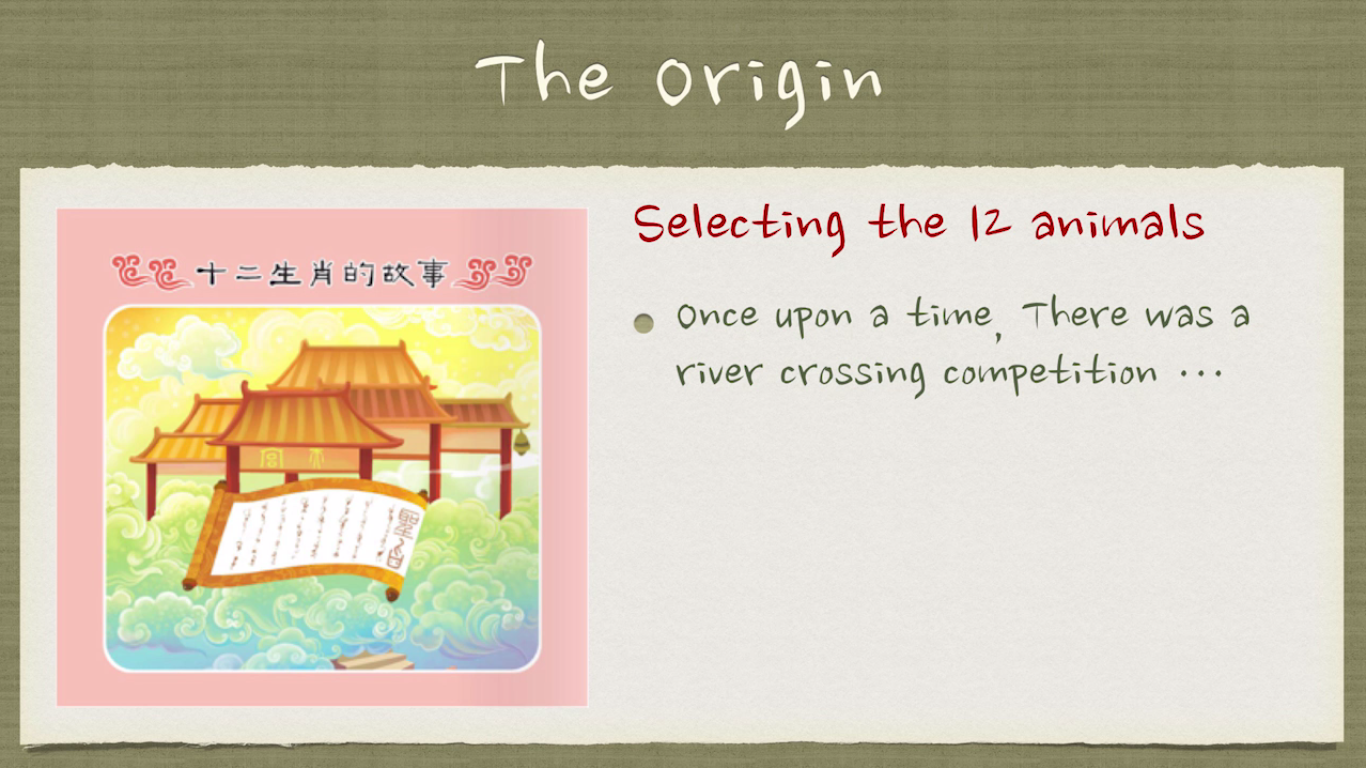
\includegraphics[width=\textwidth]{Figures/Audio.png}
        \caption{No embodiment}
        \label{fig:noembodiment}
    \end{subfigure}
    
    \begin{subfigure}{0.3\textwidth}
        \centering
        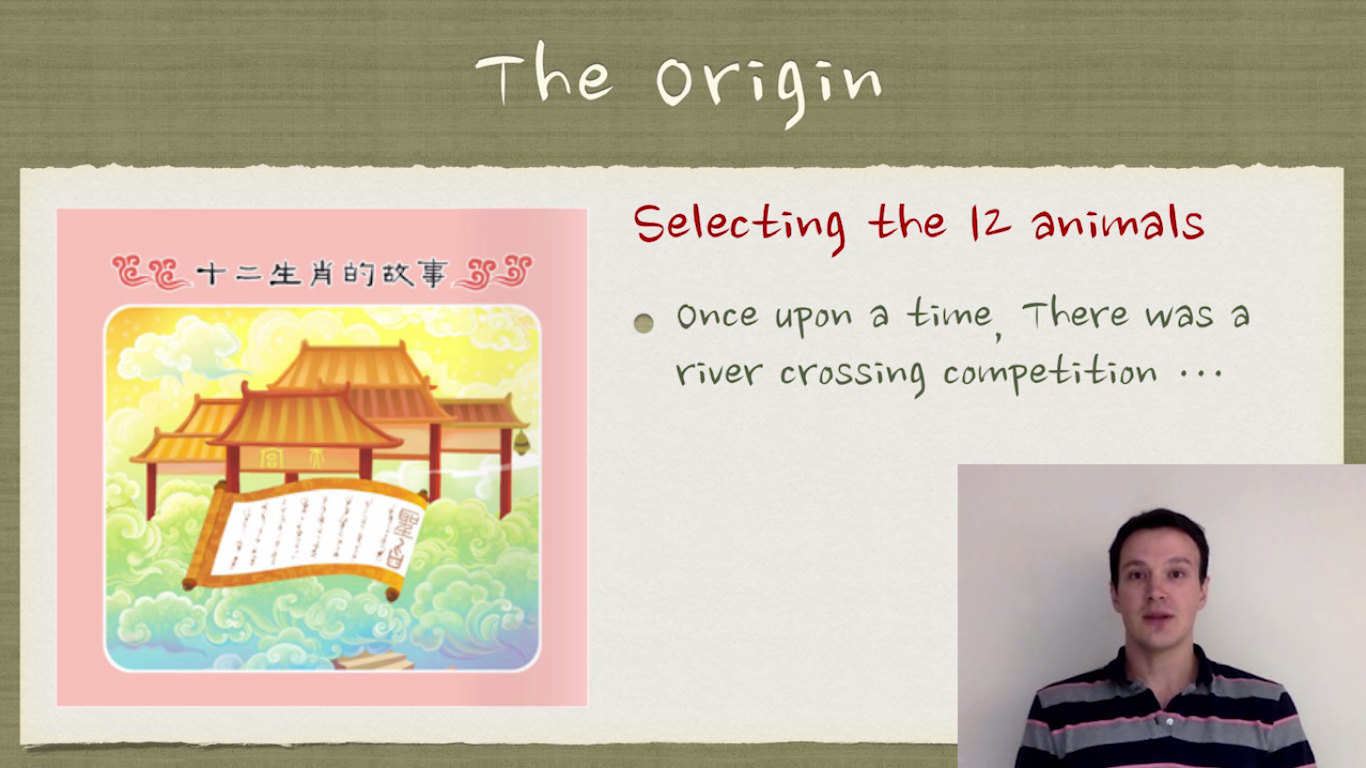
\includegraphics[width=\textwidth]{Figures/Human.png}
        \caption{Human embodiment}
        \label{fig:humanembodiment}
    \end{subfigure}
    
    \begin{subfigure}{0.3\textwidth}
        \centering
        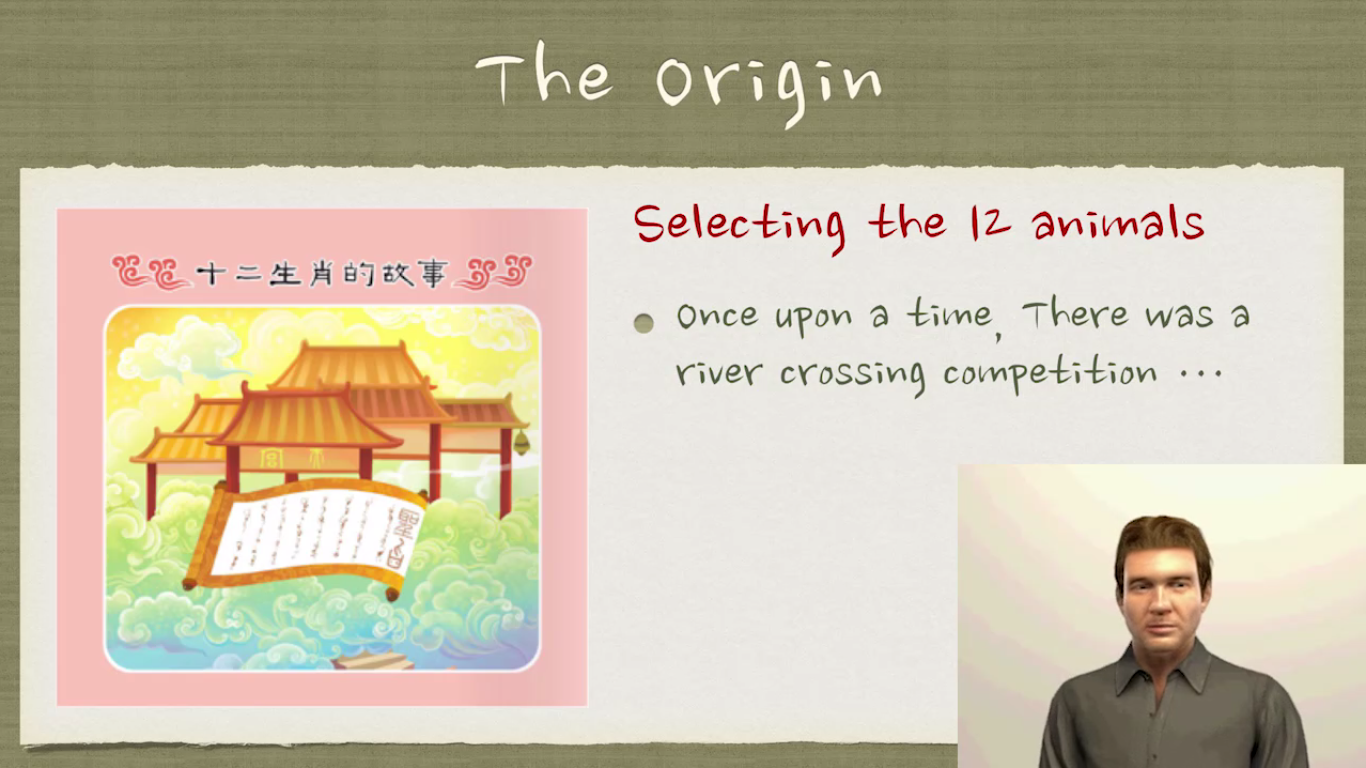
\includegraphics[width=\textwidth]{Figures/Agent.png}
        \caption{Virtual agent embodiment}
        \label{fig:virtualembodiment}
    \end{subfigure}
    \caption{Three different types of embodiment.}
    \label{fig:embodiments}
\end{figure}

\subsection{Study Design}
To test our hypotheses, we conducted a 3x1 between-participants experiment. The independent variable was the embodiment of the instructor in the lecture video, which had three levels: (1) no embodiment, (2) human embodiment, and (3) virtual agent embodiment. The three levels are described in detail below.

\begin{itemize}
\item \textit{No embodiment} - no inset frame is in the video.
\item \textit{Human embodiment} - the video has an inset frame on its lower right corner. The frame shows the face and part of the upper body of the human instructor as he gives the lecture. The inset video is a crop of the video from which the audio track was extracted. As such, the physical and lip movements of the instructor are synchronized with the audio track.
\item \textit{Virtual agent embodiment} - this is similar to the above, except that the inset frame shows a virtual agent in place of a human. We used Virtual Human Toolkit~\cite{DBLP:conf/iva/HartholtTMSSLMG13} to create the virtual agent, synchronize its lip movement with the voice in the audio track and generate some gestures.
\end{itemize}

In order to maintain consistency across participants, the three video lectures with different types of embodiment are on the same topic of the Chinese Zodiac, and of the same length of 3:40. The same lecture slides and audio track were used across all three videos. Screenshots of the three conditions can be found in Figure~\ref{fig:embodiments}. To control the effect of gender as a confounding variable, participants were stratified by gender. That is, each of the three populations had the same gender ratio.

The dependent variables included participants' recall of the lecture content and their perception of the lecture content and the instructor. 

% * <jiashen@gmail.com> 2014-12-11T04:45:41.797Z:
%
%  I'm moving the description of the embodiments from experimental procedure to design. procedure should just talk about what participants did.
%
% ^ <jiashen@gmail.com> 2014-12-15T23:30:30.592Z.
% * <jiashen@gmail.com> 2014-12-11T03:11:45.659Z:
%
%  We need to either define what's "personalized" video lecture or not use the term. I think we should just avoid it. It just confuses people and even Bilge doesn't know what it means
%
% ^ <jiashen@gmail.com> 2014-12-15T23:30:31.873Z.





\subsection{Measures}
To measure students' learning process, we utilized both objective and subjective measures.

\subsubsection{Measures of Learning Performance}
In order to measure the participant's learning performance, we asked participants to complete a post-test after watching the video lecture. The ten questions in this test were designed to measure their ability to recall the details of the lecture content regarding the Chinese Zodiac. The questions were all 5-choice MCQs with the last choice being ``I don't know''. The participants were encouraged to answer ``I don't know'' if they were not confident instead of answering randomly. The time duration that the participants spent answering the questions were recorded.

We adopted the inverse efficiency score (IES) \cite{bruyer2011combining} as the objective measure of the participant's learning performance. IES is measured as follows:

\begin{equation}
\text{IES}=\frac{\text{RT}}{\text{PC}}
\end{equation}

Here, RT corresponds to the response time (in seconds) and PC is the proportion of correct responses. IES measures how much time a participant took per correct response. A smaller IES corresponds to better performance.

\subsubsection{Measures of Learning Experience}

In order to measure the participant's learning experience, we asked participants to fill in a post-experiment questionnaire where they could rate the lecture content and the instructor on a seven-point Likert scale, 1 = Extremely disagree, 7 = Extremely agree, with 4 statements each. Statements followed items in Motivational Theory. Items of the \textit{Content Quality} scale included interestingness, topic relevance, satisfaction and meeting expectation. Items of the \textit{Instructor Satisfaction} scale included confidence, presentation, voice and drivenness.

Item reliability for both the \textit{Content Quality} scale (Cronbach's $\alpha$ = .93) and the \textit{Instructor Satisfaction} scale (Cronbach's $\alpha$ = .96) were high.

\subsection{Procedure}
The experiment was entirely conducted online. Participants were presented with a brief description of the experiment and signed a consent form. They were then given a pre-test consisting of 10 general questions about the Chinese Zodiac to test if participants had too much prior knowledge on the topic. The pre-test followed the format of the post-test - each item had an ``I don't know'' option, which participants were encouraged to choose over random guessing. Participants were then asked to provide their gender, which was used for stratification. Following that, they were presented with a video lecture that had one of the three levels of embodiment. Participants could pause or rewatch the video as they wanted, but could not return to the video after going to the next page. After watching the video, participants played a game of Sudoku for 5 minutes. This served as the distractor task that ensured that the recalling process was separated from the learning process. Finally, they took a post-test on the lecture content, followed by a post-experiment questionnaire on their subjective perception of the lecture content and the instructor.

\subsection{Participants}
A total of 40 participants took part in the experiment. 15 of these were removed for having too much prior knowledge in the Chinese Zodiac. These were participants who answered 5 or more questions in the pre-test correctly. Doing so left us with 25 participants (17 males and 8 females). 11, 10 and 4 participants were assigned the \textit{no embodiment}, \textit{human embodiment} and \textit{virtual agent embodiment} conditions respectively. All participants were recruited using a combination of Amazon Mechanical Turk and social media. Turks received \$0.50 as compensation. All participants were native English speakers.

% To evaluate if there was any difference in the perception of the embodiment of the lecturer, we asked them to rate different aspects of the lecture content and lecturer on a scale of 1 to 7. Using these results we first found the eigenvalues and plotted the scree plot. Afterwards we constructed a factor matrix using information gained from the plot. The factor matrix revealed two factors namely lecture quality and instructor satisfaction. lecture quality included: topic relevance, topic satisfaction and topic expectance. On the other hand, instructor satisfaction included confidence, presentation, voice and drive. We also calculated the Cronbach's $\alpha$~\cite{bland1997statistics}. The values were 0.93 and 0.96 for lecture quality and instructor satisfaction respectively.

\section{Results}

We utilized analysis of variance (ANOVA) to analyze our data from objective and subjective measurements.

\begin{figure}[t]
	\centering
        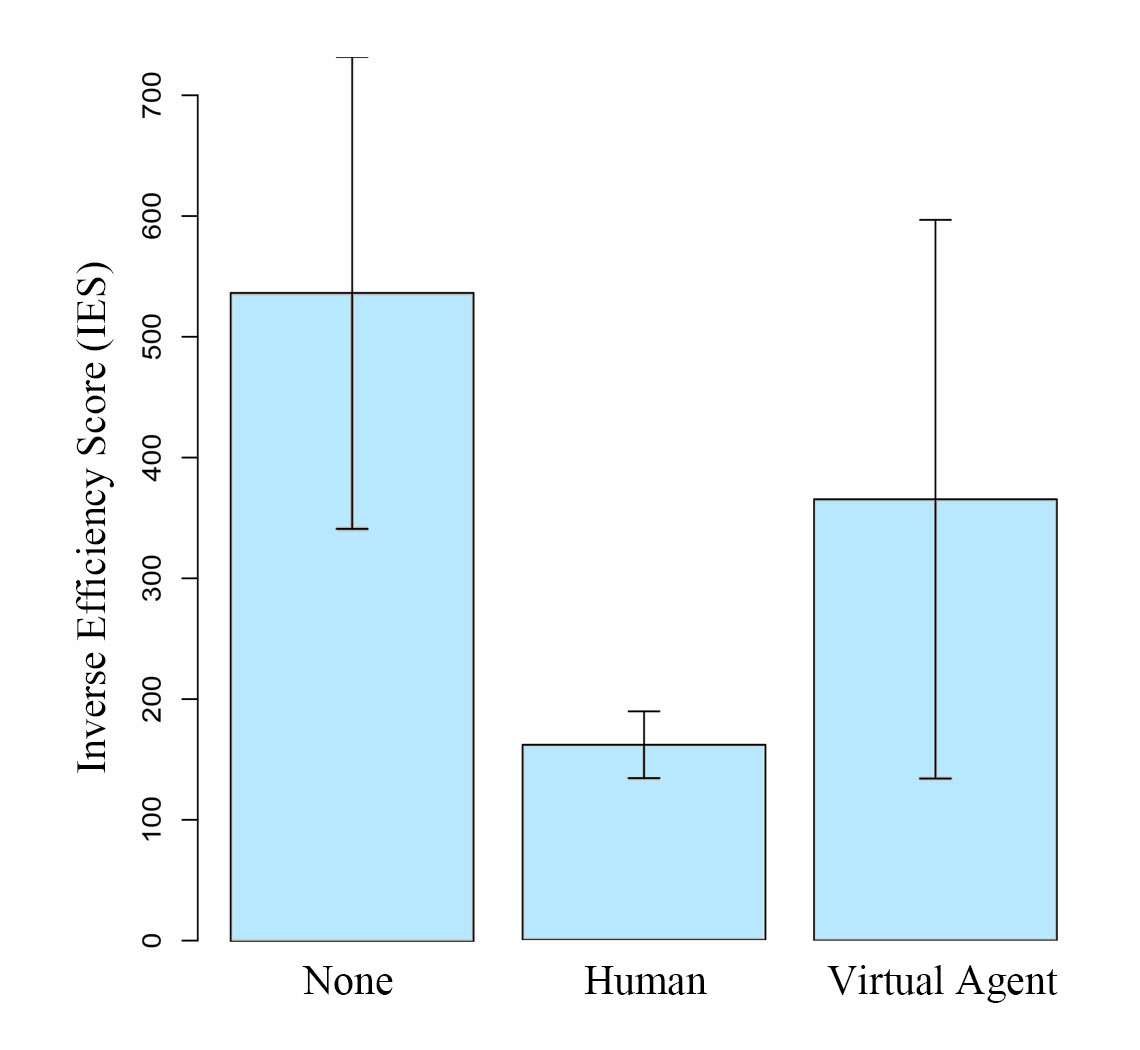
\includegraphics[width=0.4\textwidth]{Figures/IES.jpg}
        \caption{IES results for different types of embodiment.}
        \label{fig:IES}
\end{figure}

\subsection{Objective Results}

Our first hypothesis predicted that having an embodiment will lead to better learning performance for students than having no embodiment. At the same time the second hypothesis predicted that having human embodiment will yield better results than having virtual agent embodiment.

Our analysis showed that the average IES for no embodiment, human embodiment and virtual agent embodiment was 537 (\textit{SD} = 648), 162 (\textit{SD} = 87.4) and 463 (\textit{SD} = 140) respectively, as shown in Figure \ref{fig:IES}. Thus participants on average performed better when there was embodiment present in the lecture. Their performance was even better for human embodiment.

We conducted a one-way ANOVA to test whether the different types of embodiment result in different IES and found no significant difference, \textit{F}(2, 22) = 1.65, \textit{p} = .21. Post-hoc comparisons using Tukey’s HSD test revealed no significant difference in IES between the human and virtual agent embodiment, \textit{p} = .75. Therefore we did not find evidence to support Hypothesis 2, that human embodiment is better than virtual agent embodiment in terms of learning performance.

To test if having an embodiment in the lecture increases learning performance over having no embodiment, we conducted an unpaired one-tailed t-test and found a marginally significant improvement, \textit{t}(23) = 1.68, \textit{p} = .053, which supported Hypothesis 1.

The descriptive analysis suggested that a human embodiment might be better than the other types of embodiment in terms of learning performance. To test this, we conducted an unpaired one-tailed t-test and found that students learnt significantly better with a human embodiment compared to the other two types of embodiment, \textit{t}(23) = 1.73, \textit{p} = .048. 


\begin{figure}[t]
    \centering
    \begin{subfigure}{0.4\textwidth}
        \centering
        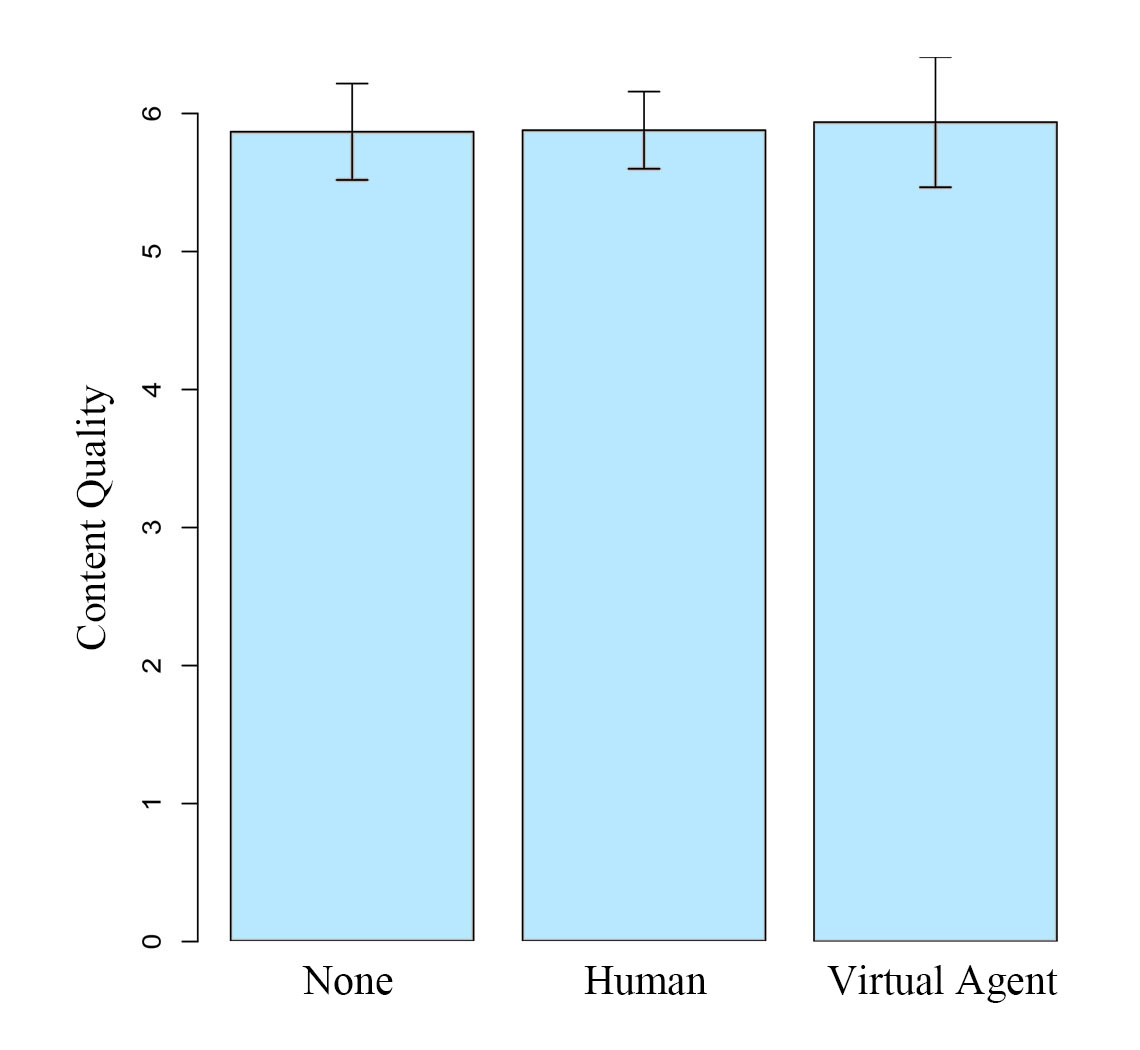
\includegraphics[width=\textwidth]{Figures/Content.jpg}
        \caption{Content quality.}
        \label{fig:Content}
    \end{subfigure}
    \begin{subfigure}{0.4\textwidth}
        \centering
        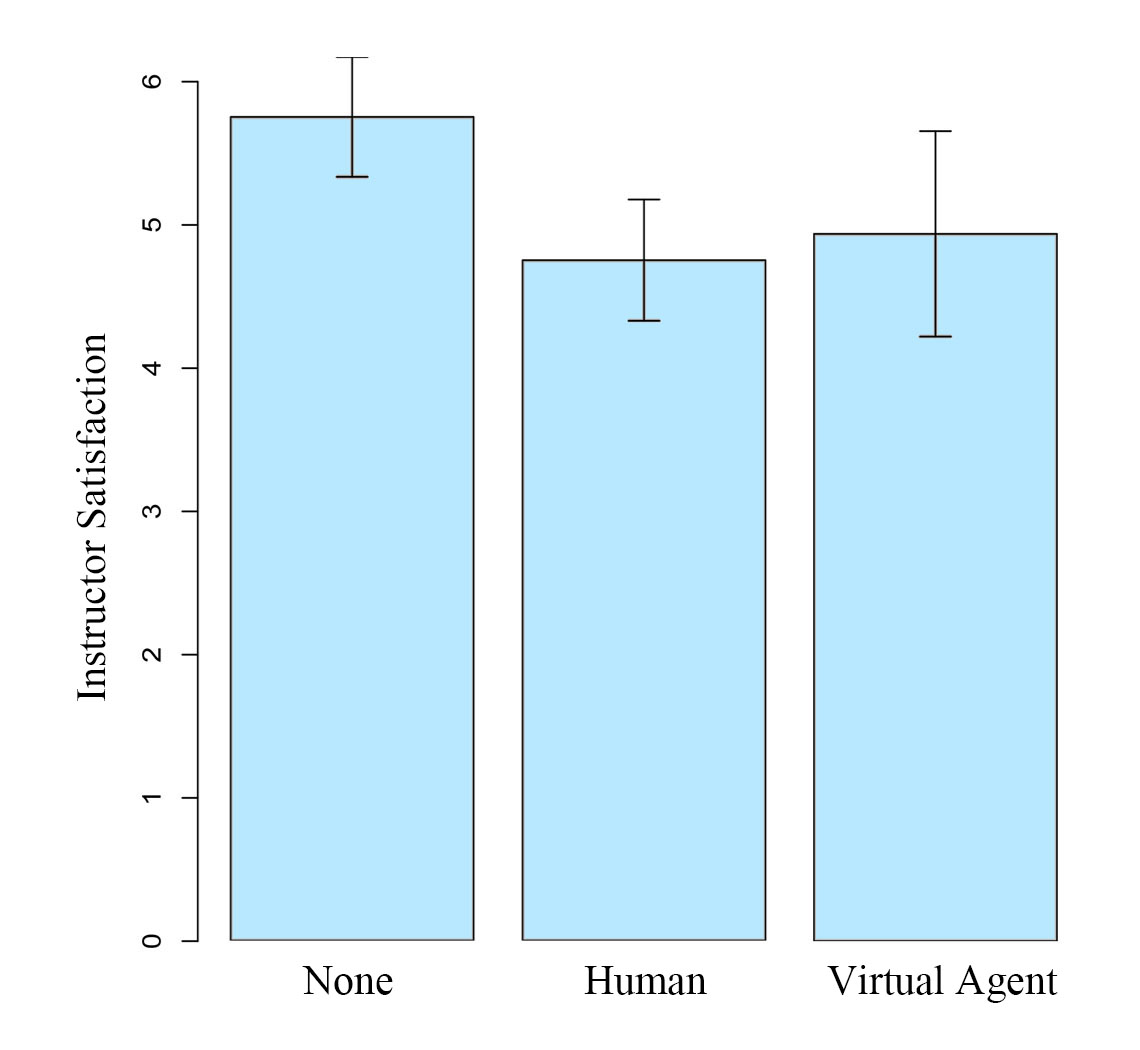
\includegraphics[width=\textwidth]{Figures/Instructor.jpg}
        \caption{Instructor satisfaction.}
        \label{fig:Instructor}
    \end{subfigure}
    
    \caption{Subjective results for different types of embodiment.}
    \label{fig:Subjective}
\end{figure}

\subsection{Subjective Results}

We conducted a one-way ANOVA to test whether the different types of embodiment result in different perceptions of the content quality and found no significant difference, \textit{F}(2, 22) = 0.008, \textit{p} = .99. We also conducted a one-way ANOVA to test whether the different types of embodiment result in different perceptions of the instructor satisfaction and again found no significant difference, \textit{F}(2, 22) = 1.49, \textit{p} = .25. This shows that participants perceived the content and the instructor almost the same regardless of embodiment. The means and standard deviations for the subjective measures are shown in Figure~\ref{fig:Subjective}.


\section{Discussion}
Our first hypothesis was that having an embodiment (of any form) in the video lecture would help people to remember the content of the lecture better. We had come up with hypothesis based on previous literature that suggested that only having audio in a video lecture is not as effective as having embodiment of the lecturer present. The average IES score in the post-test suggested that when some form of embodiment was present, the participants experienced a marginally significant improvement in learning performance.

Our second hypothesis was built upon our first hypothesis, and is that a human embodiment would be better than having a virtual agent embodiment. Even though the average IES was better for the human embodiment, it was not statistically significant.

Our third hypothesis was also not found to be well supported after statistical analyses. We had proposed that students would be more satisfied with the presence of instructor. Based on the scores for content quality and instructor satisfaction, there was no significant difference.

The lack of evidence to support two of our hypotheses suggests two important insights. Although including an inset frame of some form of embodiment improves students' learning performance over not including an inset frame, students do not perceive the lecture content or the instructor differently. Furthermore, a human embodiment does not offer a significant improve in student performance over a virtual agent embodiment. This suggests that as an alternative to filming themselves, faculty members can generate videos of virtual agents giving the lectures during post-production in order to achieve a similar effect. This reduces the additional logistic and mental preparation required to film the instructor as the lecture is being conducted.

% * <jiashen@gmail.com> 2014-12-11T05:37:48.796Z:
%
%  I still think that the paragraph above is not worded as well as it should, even after I edited it. I'll come back to it again later.
%

\section{Conclusion}
In recent years, online video lectures have grown to be a very popular medium of education. In this study, we investigated the effect of embodiment of instructor on students' learning performance and their learning experience. Unfortunately, we were only able to find evidence to support our first hypothesis. This may be due to large participant variances caused by the small sample size. The results suggest that there is some benefit for instructors to include inset frames of themselves or some generated virtual agent in their video lectures. In future studies, the sample size should be increased for more reliable results.

\section{Acknowledgments}

We would like to thank Prof. Bilge Mutlu for his mentorship, Mr. Paul Bennett who agreed to the be the instructor in our videos, and our friends who participated in the study.

% Balancing columns in a ref list is a bit of a pain because you
% either use a hack like flushend or balance, or manually insert
% a column break.  http://www.tex.ac.uk/cgi-bin/texfaq2html?label=balance
% multicols doesn't work because we're already in two-column mode,
% and flushend isn't awesome, so I choose balance.  See this
% for more info: http://cs.brown.edu/system/software/latex/doc/balance.pdf
%
% Note that in a perfect world balance wants to be in the first
% column of the last page.
%
% If balance doesn't work for you, you can remove that and
% hard-code a column break into the bbl file right before you
% submit:
%
% http://stackoverflow.com/questions/2149854/how-to-manually-equalize-columns-
% in-an-ieee-paper-if-using-bibtex
%
% Or, just remove \balance and give up on balancing the last page.
%
\balance

%\section{References format}
%References must be the same font size as other body text.
% REFERENCES FORMAT
% References must be the same font size as other body text.

\bibliographystyle{acm-sigchi}
\bibliography{sample}
\end{document}
